\documentclass[aspectratio=169]{beamer}
\usepackage[utf8]{inputenc}
\usepackage[T1]{fontenc}
\usepackage{listings}
\usepackage{xcolor}
\usepackage{tikz}
\usepackage{amssymb}  % For checkmark symbol
\usetikzlibrary{positioning, arrows.meta, shapes}

% Theme
\usetheme{Madrid}
\usecolortheme{default}

% Colors
\definecolor{teensygreen}{RGB}{0,255,136}
\definecolor{teensydark}{RGB}{10,14,39}
\definecolor{codeblue}{RGB}{86,156,214}
\definecolor{codeorange}{RGB}{206,145,120}

\setbeamercolor{structure}{fg=teensygreen!80!black}
\setbeamercolor{palette primary}{bg=teensydark,fg=white}
\setbeamercolor{palette secondary}{bg=teensygreen!70!black,fg=white}
\setbeamercolor{palette tertiary}{bg=teensydark,fg=white}

% Code styling
\lstdefinestyle{tidalstyle}{
    backgroundcolor=\color{teensydark},
    basicstyle=\ttfamily\color{white}\small,
    keywordstyle=\color{teensygreen},
    commentstyle=\color{gray},
    stringstyle=\color{codeorange},
    numberstyle=\tiny\color{gray},
    breaklines=true,
    showstringspaces=false,
    frame=single,
    rulecolor=\color{teensygreen}
}

\lstdefinestyle{cppstyle}{
    language=C++,
    backgroundcolor=\color{teensydark},
    basicstyle=\ttfamily\color{white}\footnotesize,
    keywordstyle=\color{codeblue},
    commentstyle=\color{gray}\itshape,
    stringstyle=\color{codeorange},
    numberstyle=\tiny\color{gray},
    breaklines=true,
    showstringspaces=false,
    frame=single,
    rulecolor=\color{teensygreen}
}

% Title
\title{TidalTeensy}
\subtitle{Embedded Live Coding System on Teensy 4.0}
\author{Your Name}
\institute{ENS - M2 EAS}
\date{\today}

\begin{document}

% Title slide
\begin{frame}
\titlepage
\end{frame}

% Table of contents
\begin{frame}{Outline}
\tableofcontents
\end{frame}

% ============================================================
\section{Project Overview}
% ============================================================

\begin{frame}{What is TidalTeensy?}
\begin{columns}
\column{0.5\textwidth}
\textbf{A live coding music system inspired by TidalCycles}
\begin{itemize}
    \item Runs on \textbf{Teensy 4.0} microcontroller
    \item Real-time pattern-based music generation
    \item Web-based code editor interface
    \item 8 independent channels
    \item 15 built-in instruments
    \item USB Serial + Audio output
\end{itemize}

\column{0.5\textwidth}
\begin{center}
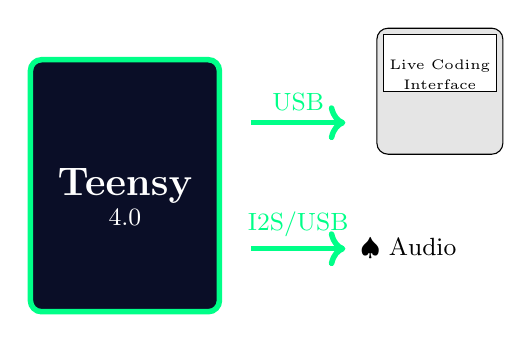
\begin{tikzpicture}[scale=0.8]
    % Teensy board
    \draw[fill=teensydark, draw=teensygreen, line width=2pt, rounded corners] 
        (0,0) rectangle (3,4);
    \node[white, font=\Large\bfseries] at (1.5,2) {Teensy};
    \node[white, font=\small] at (1.5,1.5) {4.0};
    
    % USB connection
    \draw[->, line width=2pt, teensygreen] (3.5,3) -- (5,3) 
        node[midway, above, font=\small] {USB};
    
    % Computer
    \draw[fill=gray!20, rounded corners] (5.5,2.5) rectangle (7.5,4.5);
    \draw[fill=white] (5.6,3.5) rectangle (7.4,4.4);
    \node[font=\tiny] at (6.5,3.9) {Live Coding};
    \node[font=\tiny] at (6.5,3.6) {Interface};
    
    % Audio out
    \draw[->, line width=2pt, teensygreen] (3.5,1) -- (5,1) 
        node[midway, above, font=\small] {I2S/USB};
    \node[font=\small] at (6,1) {$\spadesuit$ Audio};
\end{tikzpicture}
\end{center}
\end{columns}
\end{frame}

\begin{frame}[fragile]{Key Features}
\begin{itemize}
    \item \textbf{Pattern-based sequencing}: Tidal-style syntax for rhythm programming
    \item \textbf{Microsecond precision}: Hardware timer-based scheduling
    \item \textbf{Polyphony}: 16-voice dynamic allocation
    \item \textbf{Real-time synthesis}: On-chip DSP audio generation
    \item \textbf{Dual audio output}: I2S DAC + USB Audio simultaneously
    \item \textbf{Interactive visualizer}: Real-time event display with BPM sync
\end{itemize}

\vspace{0.5cm}
\begin{block}{Example Pattern}
\begin{lstlisting}[style=tidalstyle]
d1 bd sd hh cp        -- Drum pattern on channel 1
d2 hh*8              -- 8 hi-hats per cycle
d3 bass:c2*4         -- Bass line with multiplier
bpm 140              -- Set tempo to 140 BPM
\end{lstlisting}
\end{block}
\end{frame}

% ============================================================
\section{Architecture}
% ============================================================

\begin{frame}{System Architecture}
\begin{center}
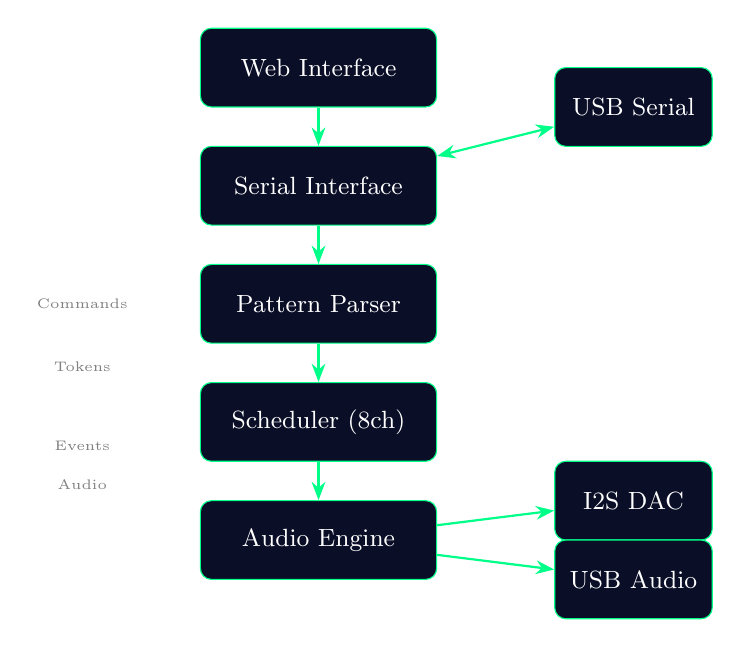
\begin{tikzpicture}[
    block/.style={rectangle, draw=teensygreen, fill=teensydark, text=white, 
                  rounded corners, minimum height=1cm, minimum width=3cm, font=\small},
    arrow/.style={->, >=Stealth, thick, teensygreen}
]
    % Layers
    \node[block] (interface) at (0,6) {Web Interface};
    \node[block] (serial) at (0,4.5) {Serial Interface};
    \node[block] (parser) at (0,3) {Pattern Parser};
    \node[block] (scheduler) at (0,1.5) {Scheduler (8ch)};
    \node[block] (audio) at (0,0) {Audio Engine};
    
    % Side components
    \node[block, minimum width=2cm] (usb) at (4,5.5) {USB Serial};
    \node[block, minimum width=2cm] (i2s) at (4,0.5) {I2S DAC};
    \node[block, minimum width=2cm] (usbaudio) at (4,-0.5) {USB Audio};
    
    % Connections
    \draw[arrow] (interface) -- (serial);
    \draw[arrow] (serial) -- (parser);
    \draw[arrow] (parser) -- (scheduler);
    \draw[arrow] (scheduler) -- (audio);
    
    \draw[arrow, <->] (serial) -- (usb);
    \draw[arrow] (audio) -- (i2s);
    \draw[arrow] (audio) -- (usbaudio);
    
    % Labels
    \node[font=\tiny, text=gray] at (-3,3) {Commands};
    \node[font=\tiny, text=gray] at (-3,2.2) {Tokens};
    \node[font=\tiny, text=gray] at (-3,1.2) {Events};
    \node[font=\tiny, text=gray] at (-3,0.7) {Audio};
\end{tikzpicture}
\end{center}
\end{frame}

% ============================================================
\section{Pattern Parser}
% ============================================================

\begin{frame}[fragile]{Pattern Parser: Tokenization}
\textbf{Role}: Convert text patterns into structured tokens

\vspace{0.3cm}
\begin{columns}
\column{0.5\textwidth}
\textbf{Input Pattern:}
\begin{lstlisting}[style=tidalstyle]
d1 bd sd hh*4 ~
\end{lstlisting}

\textbf{Recognized Elements:}
\begin{itemize}
    \item Samples: \texttt{bd, sd, hh}
    \item Multipliers: \texttt{*N}
    \item Silences: \texttt{\textasciitilde}
    \item Groups: \texttt{[...]} (future)
\end{itemize}

\column{0.5\textwidth}
\textbf{Token Structure:}
\begin{lstlisting}[style=cppstyle]
struct Token {
  char value[16];
  int multiplier;
  TokenType type;
};
\end{lstlisting}

\textbf{Output Tokens:}
\begin{itemize}
    \item \texttt{\{bd, mult=1\}}
    \item \texttt{\{sd, mult=1\}}
    \item \texttt{\{hh, mult=4\}}
    \item \texttt{\{SILENCE\}}
\end{itemize}
\end{columns}
\end{frame}

\begin{frame}[fragile]{Pattern Parser: Event Generation}
\textbf{Tokens → Events with timing information}

\vspace{0.3cm}
\begin{lstlisting}[style=cppstyle]
struct PatternEvent {
  char sample[16];      // "bd", "sine:c4", etc.
  float start;          // Position in cycle (0.0-1.0)
  float duration;       // Event duration
  float velocity;       // Volume/intensity
  bool active;          // Currently playing?
};
\end{lstlisting}

\vspace{0.3cm}
\textbf{Example}: Pattern \texttt{bd sd hh*2}
\begin{itemize}
    \item Total: 4 events (bd, sd, hh, hh)
    \item Step size: $1.0 / 4 = 0.25$
    \item \texttt{bd}: start=0.0, \texttt{sd}: start=0.25, \texttt{hh}: start=0.5, \texttt{hh}: start=0.75
\end{itemize}
\end{frame}

\begin{frame}[fragile]{Pattern Parser: Note Parsing}
\textbf{Musical notes support}: \texttt{instrument:note} format

\vspace{0.3cm}
\begin{columns}
\column{0.5\textwidth}
\textbf{Supported instruments:}
\begin{itemize}
    \item Percussion: bd, sd, hh, cp, tom, rim, cymbal
    \item Melodic: sine, saw, square, triangle, bass, lead, pad, pluck
\end{itemize}

\column{0.5\textwidth}
\textbf{Note format:}
\begin{itemize}
    \item \texttt{c4} = Middle C
    \item \texttt{d\#3} = D sharp, octave 3
    \item \texttt{gb5} = G flat, octave 5
    \item Range: \texttt{c0} to \texttt{b8}
\end{itemize}
\end{columns}

\vspace{0.3cm}
\begin{lstlisting}[style=tidalstyle]
d2 bass:c2 bass:e2 bass:g2 bass:c3    -- Bass progression
d3 sine:c4 sine:e4 sine:g4            -- Major chord
d4 pluck:a3*8                         -- Arpeggio
\end{lstlisting}
\end{frame}

% ============================================================
\section{Scheduler}
% ============================================================

\begin{frame}{Scheduler: Multi-channel Timing Engine}
\begin{columns}
\column{0.5\textwidth}
\textbf{Core Responsibilities:}
\begin{enumerate}
    \item Store patterns for 8 channels
    \item Calculate event trigger times
    \item Detect when events should fire
    \item Trigger AudioEngine synthesis
\end{enumerate}

\vspace{0.5cm}
\textbf{Timing precision:}
\begin{itemize}
    \item Uses \texttt{micros()} hardware timer
    \item Microsecond accuracy
    \item Global clock synchronization
\end{itemize}

\column{0.5\textwidth}
\begin{center}
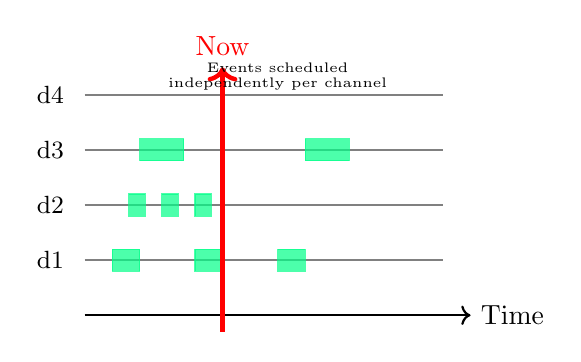
\begin{tikzpicture}[scale=0.7]
    % Timeline
    \draw[->, thick] (0,0) -- (7,0) node[right] {Time};
    
    % Channels
    \foreach \y/\ch in {1/d1, 2/d2, 3/d3, 4/d4} {
        \draw[thick, gray] (0,\y) -- (6.5,\y);
        \node[left, font=\small] at (-0.2,\y) {\ch};
    }
    
    % Events as boxes
    \filldraw[teensygreen, opacity=0.7] (0.5,0.8) rectangle (1.0,1.2);
    \filldraw[teensygreen, opacity=0.7] (2.0,0.8) rectangle (2.5,1.2);
    \filldraw[teensygreen, opacity=0.7] (3.5,0.8) rectangle (4.0,1.2);
    
    \filldraw[teensygreen, opacity=0.7] (0.8,1.8) rectangle (1.1,2.2);
    \filldraw[teensygreen, opacity=0.7] (1.4,1.8) rectangle (1.7,2.2);
    \filldraw[teensygreen, opacity=0.7] (2.0,1.8) rectangle (2.3,2.2);
    
    \filldraw[teensygreen, opacity=0.7] (1.0,2.8) rectangle (1.8,3.2);
    \filldraw[teensygreen, opacity=0.7] (4.0,2.8) rectangle (4.8,3.2);
    
    % Playhead
    \draw[->, ultra thick, red] (2.5,-0.3) -- (2.5,4.5) node[above] {Now};
    
    \node[font=\tiny] at (3.5,4.5) {Events scheduled};
    \node[font=\tiny] at (3.5,4.2) {independently per channel};
\end{tikzpicture}
\end{center}
\end{columns}
\end{frame}

\begin{frame}[fragile]{Scheduler: Algorithm}
\textbf{Update Loop} (called every audio block):

\begin{lstlisting}[style=cppstyle]
void Scheduler::update(unsigned long currentMicros) {
  // Calculate cycle progress (0.0-1.0)
  float cyclePosition = (currentMicros % cycleDurationMicros) 
                        / (float)cycleDurationMicros;
  
  // Check each channel
  for (int ch = 0; ch < 8; ch++) {
    for (int i = 0; i < eventCount[ch]; i++) {
      PatternEvent& evt = events[ch][i];
      
      // Should this event trigger now?
      if (!eventTriggered[ch][i] && 
          cyclePosition >= evt.start) {
        
        triggerEvent(ch, evt); // Tell AudioEngine
        eventTriggered[ch][i] = true;
      }
    }
    
    // Reset flags at cycle end
    if (cyclePosition < lastPosition[ch]) {
      resetTriggeredFlags(ch);
    }
  }
}
\end{lstlisting}
\end{frame}

\begin{frame}{Scheduler: BPM and Timing}
\textbf{Cycle duration calculation:}

\begin{equation}
T_{cycle} = \frac{60,000,000 \times 4}{BPM} \text{ microseconds}
\end{equation}

\vspace{0.3cm}
\begin{itemize}
    \item 1 cycle = 4 beats (1 bar in 4/4 time)
    \item Default: 120 BPM → $T_{cycle} = 2,000,000$ µs (2 seconds)
    \item At 180 BPM → $T_{cycle} = 1,333,333$ µs (1.33 seconds)
\end{itemize}

\vspace{0.5cm}
\textbf{Event trigger time:}
\begin{equation}
T_{event} = T_{cycle} \times \text{event.start}
\end{equation}

\vspace{0.3cm}
Example: Event at position 0.5 with 120 BPM triggers at 1,000,000 µs (1 second into cycle)
\end{frame}

% ============================================================
\section{Audio Engine}
% ============================================================

\begin{frame}{Audio Engine: Sound Synthesis}
\textbf{Built on Teensy Audio Library}

\vspace{0.3cm}
\begin{columns}
\column{0.5\textwidth}
\textbf{Architecture:}
\begin{itemize}
    \item 16 voices polyphony
    \item Dynamic voice allocation
    \item Per-voice ADSR envelope
    \item Real-time synthesis
    \item 44.1 kHz, 16-bit audio
\end{itemize}

\vspace{0.3cm}
\textbf{Output routing:}
\begin{itemize}
    \item I2S DAC (physical output)
    \item USB Audio (to computer)
    \item Both outputs simultaneous
\end{itemize}

\column{0.5\textwidth}
\begin{center}
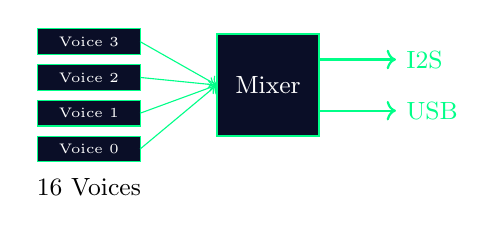
\begin{tikzpicture}[scale=0.65]
    % Voice pool
    \foreach \i in {0,...,3} {
        \draw[fill=teensydark, draw=teensygreen] 
            (0,\i*0.7) rectangle (2,\i*0.7+0.5);
        \node[white, font=\tiny] at (1,\i*0.7+0.25) {Voice \i};
    }
    \node[font=\small] at (1,-0.5) {16 Voices};
    
    % Mixer
    \draw[fill=teensydark, draw=teensygreen, thick] 
        (3.5,0.5) rectangle (5.5,2.5);
    \node[white, font=\small] at (4.5,1.5) {Mixer};
    
    % Outputs
    \draw[->, thick, teensygreen] (5.5,2) -- (7,2) 
        node[right, font=\small] {I2S};
    \draw[->, thick, teensygreen] (5.5,1) -- (7,1) 
        node[right, font=\small] {USB};
    
    % Connections
    \foreach \i in {0,...,3} {
        \draw[->, teensygreen] (2,\i*0.7+0.25) -- (3.5,1.5);
    }
\end{tikzpicture}
\end{center}
\end{columns}
\end{frame}

\begin{frame}{Audio Engine: Instrument Types}
\begin{columns}
\column{0.5\textwidth}
\textbf{Percussion (7 instruments):}
\begin{itemize}
    \item \textbf{bd}: Bass drum (kick)
    \item \textbf{sd}: Snare drum
    \item \textbf{hh}: Hi-hat
    \item \textbf{cp}: Clap
    \item \textbf{tom}: Tom drum
    \item \textbf{rim}: Rimshot
    \item \textbf{cymbal}: Crash cymbal
\end{itemize}

\column{0.5\textwidth}
\textbf{Melodic (8 instruments):}
\begin{itemize}
    \item \textbf{sine}: Pure sine wave
    \item \textbf{saw}: Sawtooth (bright)
    \item \textbf{square}: Square wave (hollow)
    \item \textbf{triangle}: Triangle wave (soft)
    \item \textbf{bass}: Sub-bass synth
    \item \textbf{lead}: Lead synth
    \item \textbf{pad}: Pad synth (slow attack)
    \item \textbf{pluck}: Plucked string
\end{itemize}
\end{columns}

\vspace{0.5cm}
\textbf{Total: 15 instruments} with unique timbres and ADSR envelopes
\end{frame}

\begin{frame}[fragile]{Audio Engine: Synthesis Example}
\textbf{Bass Drum Generation:}

\begin{lstlisting}[style=cppstyle]
void AudioEngine::generateKick(int voiceIndex, float velocity) {
  Voice& v = voices[voiceIndex];
  
  // Pitch sweep: 150Hz -> 50Hz
  v.waveform.frequency(150.0f);
  v.waveform.begin(velocity, 50.0f, WAVEFORM_SINE);
  
  // Short, punchy envelope
  v.envelope.attack(0.5);   // 0.5ms attack
  v.envelope.decay(150);    // 150ms decay
  v.envelope.sustain(0.0);  // No sustain
  v.envelope.release(50);   // 50ms release
  
  v.waveform.frequencyModulation(2.0); // FM for punch
  v.isActive = true;
}
\end{lstlisting}

\vspace{0.3cm}
\textbf{Result}: Punchy kick drum with pitch envelope and FM synthesis
\end{frame}

\begin{frame}[fragile]{Audio Engine: Note Frequency Calculation}
\textbf{MIDI-style note to frequency conversion:}

\begin{lstlisting}[style=cppstyle]
float AudioEngine::noteToFreq(const char* note) {
  // Parse note (e.g., "c4", "d#3", "gb5")
  char noteName = note[0];
  int octave = note[strlen(note)-1] - '0';
  
  // Calculate semitone (c=0, c#=1, d=2, ...)
  int semitone = noteToSemitone(noteName);
  
  // Check for sharp/flat
  if (note[1] == '#' || note[1] == 's') semitone++;
  if (note[1] == 'b') semitone--;
  
  // MIDI note number: 12*octave + semitone
  int midiNote = 12 * octave + semitone;
  
  // A4 (440Hz) is MIDI note 69
  return 440.0f * pow(2.0f, (midiNote - 69) / 12.0f);
}
\end{lstlisting}

\textbf{Example}: \texttt{c4} → MIDI 60 → 261.63 Hz (Middle C)
\end{frame}

% ============================================================
\section{Web Interface}
% ============================================================

\begin{frame}{Web Interface: Live Coding Editor}
\begin{columns}
\column{0.5\textwidth}
\textbf{Features:}
\begin{itemize}
    \item Multi-line code editor
    \item Real-time syntax validation
    \item Line-by-line evaluation
    \item Visual line indicators:
    \begin{itemize}
        \item Green: Sent to Teensy
        \item Orange: Modified
        \item Red: Syntax error
    \end{itemize}
    \item Keyboard shortcuts
    \item Quick command buttons
\end{itemize}

\column{0.5\textwidth}
\textbf{Technology:}
\begin{itemize}
    \item Web Serial API
    \item Direct USB communication
    \item No middleware required
    \item Chrome/Edge/Opera only
    \item 115200 baud rate
\end{itemize}

\vspace{0.3cm}
\textbf{Shortcuts:}
\begin{itemize}
    \item Ctrl+Enter: Evaluate all
    \item Shift+Enter: Evaluate line
    \item Ctrl+.: Stop all patterns
    \item Ctrl+L: Clear console
\end{itemize}
\end{columns}
\end{frame}

\begin{frame}{Real-time Visualizer}
\textbf{8-channel event visualization with BPM synchronization}

\vspace{0.3cm}
\begin{center}
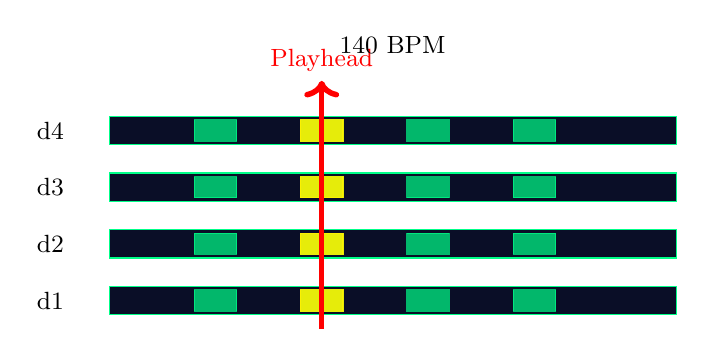
\begin{tikzpicture}[scale=0.9]
    % Timeline bars for 8 channels
    \foreach \i in {1,...,4} {
        % Channel label
        \node[left, font=\small] at (0,\i*0.8-0.4) {d\i};
        
        % Timeline bar
        \draw[fill=teensydark, draw=teensygreen] 
            (0.5,\i*0.8-0.6) rectangle (8.5,\i*0.8-0.2);
        
        % Event boxes
        \foreach \x in {1,2,3,4} {
            \filldraw[teensygreen, opacity=0.7] 
                (\x*1.5+0.2,\i*0.8-0.55) rectangle (\x*1.5+0.8,\i*0.8-0.25);
        }
        
        % Active event (yellow)
        \filldraw[yellow, opacity=0.9] 
            (3.2,\i*0.8-0.55) rectangle (3.8,\i*0.8-0.25);
    }
    
    % Playhead
    \draw[->, ultra thick, red, line width=2pt] (3.5,0) -- (3.5,3.5);
    \node[above, red, font=\small] at (3.5,3.5) {Playhead};
    
    % BPM indicator
    \node[font=\small] at (4.5,4) {140 BPM};
\end{tikzpicture}
\end{center}

\vspace{0.3cm}
\textbf{Features:}
\begin{itemize}
    \item Event boxes show pattern structure
    \item Playhead loops synchronized with BPM
    \item Active events highlighted in yellow
    \item Supports multipliers (\texttt{hh*8} shows 8 boxes)
    \item Toggle on/off with button
\end{itemize}
\end{frame}

% ============================================================
\section{Performance \& Results}
% ============================================================

\begin{frame}{System Performance}
\begin{columns}
\column{0.5\textwidth}
\textbf{Teensy 4.0 Specifications:}
\begin{itemize}
    \item ARM Cortex-M7 @ 600 MHz
    \item 1 MB RAM
    \item 2 MB Flash
    \item Hardware floating-point
    \item DMA audio subsystem
\end{itemize}

\vspace{0.3cm}
\textbf{Audio Performance:}
\begin{itemize}
    \item Sample rate: 44.1 kHz
    \item Bit depth: 16-bit
    \item Latency: < 3 ms
    \item CPU usage: ~30\% typical
\end{itemize}

\column{0.5\textwidth}
\textbf{Capabilities:}
\begin{itemize}
    \item 16 simultaneous voices
    \item 8 independent channels
    \item Up to 64 events per channel
    \item Microsecond timing precision
    \item BPM range: 40-300
\end{itemize}

\vspace{0.3cm}
\textbf{Memory Usage:}
\begin{itemize}
    \item Pattern storage: ~25 KB
    \item Audio buffers: 50 KB
    \item Code: ~180 KB
    \item Remaining: ~750 KB
\end{itemize}
\end{columns}
\end{frame}

\begin{frame}[fragile]{Example Session}
\begin{block}{Live Coding Workflow}
\begin{lstlisting}[style=tidalstyle]
-- Start with basic drums
d1 bd sd hh cp
bpm 120

-- Add hi-hat pattern
d2 hh*8

-- Bass line
d3 bass:c2 bass:c2 bass:e2 bass:g2

-- Lead melody
d4 pluck:c4 pluck:e4 pluck:g4 pluck:c5

-- Increase tempo
bpm 140

-- Add variation
d2 hh*16
d3 bass:c2*8

-- Stop specific channel
d4 silence
\end{lstlisting}
\end{block}
\end{frame}

% ============================================================
\section{Conclusion}
% ============================================================

\begin{frame}{Achievements}
\begin{itemize}
    \item[\checkmark] Fully functional embedded live coding system
    \item[\checkmark] Real-time pattern parsing and scheduling
    \item[\checkmark] Multi-channel polyphonic synthesis
    \item[\checkmark] Professional web-based interface
    \item[\checkmark] Real-time visualization with BPM sync
    \item[\checkmark] Dual audio output (I2S + USB)
    \item[\checkmark] Microsecond-precision timing
\end{itemize}

\vspace{0.5cm}
\textbf{Key Innovation:}
Complete live coding music system on a \$25 microcontroller with no external computer required for synthesis
\end{frame}

\begin{frame}{Future Improvements}
\textbf{Planned Features:}
\begin{enumerate}
    \item \textbf{Effects}: Filters, reverb, delay, distortion
    \item \textbf{Euclidean patterns}: \texttt{bd(3,8)} notation
    \item \textbf{Pattern functions}: \texttt{every}, \texttt{sometimes}, \texttt{slow}, \texttt{fast}
    \item \textbf{Groups}: \texttt{[bd sd]*2} syntax
    \item \textbf{WAV samples}: SD card sample playback
    \item \textbf{MIDI output}: Control external synthesizers
    \item \textbf{Variable duration}: Note-level timing control
    \item \textbf{Velocity control}: Per-note dynamics
\end{enumerate}

\vspace{0.5cm}
\textbf{Advanced Features:}
\begin{itemize}
    \item Probability patterns
    \item Pattern transformations
    \item Multi-pattern synchronization
\end{itemize}
\end{frame}

\begin{frame}{Conclusion}
\begin{center}
\Large
\textbf{TidalTeensy demonstrates that powerful live coding systems can run on embedded hardware}

\vspace{1cm}
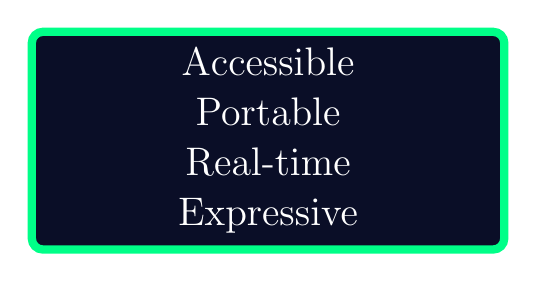
\begin{tikzpicture}
    \node[draw=teensygreen, line width=3pt, rounded corners, 
          fill=teensydark, text=white, minimum width=6cm, minimum height=2cm] {
        \Large
        \begin{tabular}{c}
        Accessible \\
        Portable \\
        Real-time \\
        Expressive
        \end{tabular}
    };
\end{tikzpicture}

\vspace{1cm}
\normalsize
Thank you for your attention!

\vspace{0.5cm}
\textit{Questions?}
\end{center}
\end{frame}

\end{document}
